\documentclass[10pt,conference]{IEEEtran}
\usepackage{graphicx}
\usepackage{amsmath}
\usepackage{amssymb}
\usepackage{booktabs}
\usepackage{array}
\usepackage[hyphens]{url}
\usepackage{cite}
\usepackage{stfloats}
\usepackage{balance}
\renewcommand{\arraystretch}{1.15}
\newcommand{\unit}[1]{\,\mathrm{#1}}

\begin{document}

\title{A Measurement Study of Automated Containment\\for Compromised Kubernetes Workloads:\\An eBPF-Based Cross-Layer Comparison}

\author{}

\maketitle
\begin{center}
\textbf{Dr. Girish L \quad (Project Guide)} \\
Associate Professor \& HOD, Artificial Intelligence and Data Science \\
Shridevi Institute of Engineering and Technology, Tumkur, India \\
girish.l@shrideviengineering.org \\ \quad \\
\textbf{D V Sharath Chandra, Moulya H A, Naveen S, Praveen D} \\
Student, Artificial Intelligence and Data Science, Shridevi Institute of Engineering and Technology, Tumkur \\
sharath9143@gmail.com, moulyaha19@gmail.com, naveen.siddappa44@gmail.com, praveen.durgesh06@gmail.com
\end{center}

\begin{abstract}
Automated runtime-threat response is usually judged by \emph{detection}, but its value depends on what happens after the alert. We measure five containment mechanisms in Kubernetes against the same attacks: pod termination and egress isolation via Falco Talon, in-kernel process termination with Tetragon, LSM blocking with KubeArmor, and in-application self-protection (RASP). On a single-node k3s testbed, each applicable mechanism-attack pair ran 20 times with fresh pods under steady benign load, timed on one clock, no runs discarded. Detection was not the bottleneck: Falco alerted about 2\,ms after the kernel event, with no false positives in 2 hours of benign traffic. Pod termination returned from the Kubernetes API in 0.02--0.10\,s, yet the attacker's process ran on for about 2\,s, completed 2--3 of 8 steps, re-compromised the replacement pod every time, and its logs were lost. Egress isolation stopped an outbound-dependent attacker after 1 of 8 steps but did nothing against an inbound HTTP attack. Tetragon stopped the attacker within 0.09\,s before any step completed, killing the shell on spawn before any of thirteen MITRE-tagged techniques from a public suite ran. KubeArmor could not block a shell on an Alpine image without blocking every BusyBox tool, and blocked without raising alerts. Under abuse, tripping the response six times a minute kept the service unavailable 225 of 300\,s with in-kernel termination, while a minimum-healthy-replicas guard removed the outage. Tetragon added under 0.1\,ms to p99 at 2{,}500\,requests/s; KubeArmor used about 1.2 extra whole-host cores. No mechanism wins on speed, durability, and cost together, which argues for a layered response; configurations, scripts, and raw run data are released.
\end{abstract}

\begin{IEEEkeywords}
Kubernetes, runtime security, automated containment, eBPF, Falco, Falco Talon, Tetragon, KubeArmor, pod termination, forensic evidence, denial of service, cloud-native security.
\end{IEEEkeywords}

\section{Introduction}
Containers, orchestrators, and automated pipelines let teams ship changes within minutes, but pods start, stop, and move continuously. Scanning source code or a built image happens before the workload runs and says nothing about its behaviour afterwards. A container image with no known critical vulnerabilities can still be abused through a logic flaw, a leaked credential, or a vulnerability that was unknown at scan time. Runtime security closes that gap by watching system calls, process creation, and file access while the software executes. eBPF has become a common foundation for it because eBPF programs can attach to kernel events without an out-of-tree kernel module~\cite{ebpf}. Recent studies compare eBPF-based tools such as Falco, Tetragon, Tracee, and KubeArmor~\cite{her2025,syairozi2025}.

Detection alone is not enough. An alert nobody sees, or that arrives without a way to \emph{contain} the workload, leaves the attacker time to act. Most published work reports detection rate, false positives, or mean time to detect; it rarely measures what happens between the alert and the attacker actually stopping. This paper treats the whole chain as one system, image scanning in CI, kernel-level detection, event forwarding, observability, and automated containment, and it measures the containment step directly: once a container is compromised, does the attacker's process actually stop, how fast, how durably, at what cost to normal users, and can the response itself be abused.

An earlier version of this work described the architecture and a measurement protocol but reported no figures. This version reports the measurements. The contributions are:
\begin{enumerate}
\item An open, single-node testbed that integrates eBPF detection (Falco), alert forwarding (Falcosidekick), observability (Prometheus, Loki), and four response layers (Falco Talon, Tetragon, KubeArmor, in-app RASP) in one Kubernetes cluster, used as the common platform for every measurement below.
\item To our knowledge, the first measurement-based, cross-layer comparison of automated \emph{containment} (not detection) for a compromised Kubernetes workload, covering five containment mechanisms across four enforcement layers against a detect-only baseline under one protocol, with every claim tied to a released artifact.
\item Three findings that, to our knowledge, have not been reported together in prior work: a multi-second gap between API-level and process-level containment; that the response mechanism is itself a denial-of-service surface; and that in-kernel enforcement contains attacks early enough to blind the detection pipeline.
\item A steady-state cost comparison showing that the overhead ranking inverts the protection ranking.
\item A reproducible evaluation protocol, including an established public attack suite mapped to MITRE ATT\&CK, with all configurations, scripts, and raw run data released.
\end{enumerate}

The remainder is organised as follows. Section~\ref{sec:related} reviews background and related work; Section~\ref{sec:threat} the threat model and design goals; Section~\ref{sec:arch} the architecture; Section~\ref{sec:impl} the implementation; Section~\ref{sec:ml} a planned learned-scoring layer (future work); Section~\ref{sec:status} the implementation status; Section~\ref{sec:method} the evaluation methodology and formulas; Section~\ref{sec:results} the results; Section~\ref{sec:discuss} discussion; Section~\ref{sec:limits} limitations; and Section~\ref{sec:road} the roadmap.

\section{Background and Related Work}\label{sec:related}
\subsection{Building Blocks}
\textbf{eBPF} lets small programs run in the kernel after a verifier has checked that they terminate and access memory safely~\cite{ebpf}. Attached to tracepoints or kprobes, they observe system calls and pass events to user space through ring buffers. \textbf{Falco} evaluates such events against declarative rules and emits structured alerts~\cite{falco}; its modern eBPF driver attaches without a separate kernel module. \textbf{Falcosidekick} fans alerts out to metrics and notification back ends~\cite{falcosidekick}. \textbf{Falco Talon} consumes those alerts and executes response actions such as terminating a pod through the Kubernetes API~\cite{talon}. \textbf{Tetragon} and \textbf{KubeArmor} enforce in the kernel: Tetragon can send \texttt{SIGKILL} from a kprobe~\cite{tetragon}, and KubeArmor compiles policies to an LSM enforcer (BPF-LSM or AppArmor)~\cite{kubearmor}. \textbf{Trivy} scans images for known vulnerabilities~\cite{trivy}; \textbf{Prometheus}~\cite{prometheus} and \textbf{Grafana/Loki}~\cite{loki} provide metrics and logs; \textbf{GitHub Actions}~\cite{ghactions} and \textbf{Jenkins}~\cite{jenkins} drive the build stage.

\subsection{Related Studies}
Her et al.\ compare KubeArmor, Falco, Tetragon, and Tracee for eBPF-based system security in cloud-native environments~\cite{her2025}. Syairozi and Arizal evaluate three eBPF tools on Kubernetes using mean time to detect, detection rate, false-positive rate, and resource usage~\cite{syairozi2025}. Ghimire et al.\ present eBPF-PATROL, an agent targeting syscall- and process-level enforcement with reported overhead under 2.5\,\%~\cite{ghimire2025}. Rezvani et al.\ study how far eBPF syscall tracing alone reconstructs request-level latency metrics~\cite{rezvani2024}. Chernyshev et al.\ review the cloud-native attack surface~\cite{chernyshev2021}. For learned detection, Zhang and Chen apply an isolation forest to eBPF-collected resource usage~\cite{zhang2023}, and Anand et al.\ combine eBPF with machine learning against denial-of-service attacks~\cite{anand2025}; the isolation forest follows Liu et al.~\cite{iforest}. Broader surveys map the container attack surface and its defenses: Wong et al.\ apply STRIDE threat modeling to the container ecosystem~\cite{wong2023}, and Haq et al.\ systematize Docker attack and defense mechanisms~\cite{haq2024}. Measurement studies of container security predate ours: Lin et al.\ built a 223-exploit dataset and measured how many succeed under default isolation~\cite{lin2018}, but they study image- and kernel-level exploits, not automated runtime response. On detection technique, host-based intrusion detection from system calls is a long-standing line~\cite{liu2018,bridges2019}, recently adapted to containers with learned models over contextualized syscalls~\cite{elkhairi2022}. Closest to a response mechanism, Abbas et al.\ detect container escapes from provenance graphs~\cite{abbas2022} and Chen et al.\ from a dependency graph~\cite{chen2024}, but both stop at detection and do not compare enforcement actions. In-application self-protection has been framed as complementary rather than stand-alone~\cite{cisar2016}, and a recent empirical study found a RASP tool prevented only injection attacks in a large Java system~\cite{seth2025}, matching our finding that app-level defense is blind to OS-level activity. These works evaluate \emph{detection} or a single tool, and none compares the containment \emph{response} across layers. Table~\ref{tab:related} positions the closest studies against ours: we measure \emph{containment} across five mechanisms and four enforcement layers under one protocol, and quantify the cost and abuse of the response itself.

\begin{table*}[t]
\caption{This work versus the closest prior studies. No prior study compares the containment \emph{response} across enforcement layers or measures the response itself as a denial-of-service surface.}
\label{tab:related}
\centering
\begin{tabular}{llllcc}
\toprule
Study & Subject & Layer & Emphasis & Response abuse & Overhead\\
\midrule
Her et al.~\cite{her2025}          & 4 eBPF tools    & Kernel          & Detection + enforcement & No  & Yes\\
Syairozi \& Arizal~\cite{syairozi2025} & 3 eBPF tools & Kernel          & Detection               & No  & Yes\\
Ghimire et al.~\cite{ghimire2025}  & Single agent    & Syscall/process & Enforcement             & No  & Yes\\
Abbas et al.~\cite{abbas2022}      & Escape detector & Provenance      & Detection               & No  & Yes\\
Chen et al.~\cite{chen2024}        & Escape detector & File/provenance & Detection               & No  & --\\
El Khairi et al.~\cite{elkhairi2022} & Syscall IDS   & Syscall         & Detection               & No  & Yes\\
Seth et al.~\cite{seth2025}        & RASP/IAST tools & Application     & Detection + prevention  & No  & --\\
Zhang \& Chen~\cite{zhang2023}     & Anomaly model   & Resource usage  & Detection               & No  & No\\
Lin et al.~\cite{lin2018}          & 223 exploits    & Kernel/isolation & Attack study           & No  & No\\
\midrule
\textbf{This work} & \textbf{5 mechanisms} & \textbf{API, kernel, LSM, app} & \textbf{Containment comparison} & \textbf{Yes} & \textbf{Yes}\\
\bottomrule
\end{tabular}
\end{table*}

\section{Threat Model and Design Goals}\label{sec:threat}
\subsection{Threat Model}
The attacker is a workload already running in the cluster, or an attacker who has achieved code execution inside a container of the application, for example through a vulnerable dependency or an injection flaw. The attacker attempts unauthorized process execution (such as spawning a shell), access to sensitive files, planting or executing new binaries, privilege escalation, or container escape. We assume the Kubernetes control plane and the host kernel are not yet compromised, and that Falco's own process and its rules are not tampered with. We do not consider attacks that evade syscall-level visibility (purely in-memory logic that makes no monitored calls), attacks on the CI system itself, or supply-chain compromise of the base images beyond what Trivy reports.

\subsection{Design Goals}
\begin{itemize}
\item \textbf{Coverage across phases.} Findings from the build stage and behaviour at runtime should both be visible.
\item \textbf{Modularity.} Detection, forwarding, observability, and response can each be replaced independently.
\item \textbf{Repeatable triggers.} The application exposes harmless endpoints that reproduce each monitored behaviour, so evaluation does not depend on real malware; an established public suite supplements them.
\item \textbf{Bounded automation.} Automated actions should be limited, logged, and reversible where possible.
\end{itemize}

\begin{table}[t]
\caption{Division of responsibility among components}
\label{tab:resp}
\centering
\begin{tabular}{@{}lll@{}}
\toprule
Component & Phase & Role\\
\midrule
Trivy & Build & Known-vulnerability report on images\\
Falco + eBPF & Run & Rule-based detection from kernel events\\
Falcosidekick & Run & Alert fan-out and metrics\\
Falco Talon & Run & Kubernetes-level response (M1, M2)\\
Tetragon & Run & In-kernel \texttt{SIGKILL} response (M3)\\
KubeArmor & Run & LSM block response (M4)\\
RASP layer & Run & In-application lockdown (M5)\\
Prom./Grafana/Loki & Run & Metrics, dashboards, logs\\
Learned scoring (future work) & Run (plan) & Score behaviour no rule anticipates\\
\bottomrule
\end{tabular}
\end{table}

\section{System Architecture}\label{sec:arch}
Fig.~\ref{fig:arch} shows the pipeline. Source pushed to \texttt{main} triggers a workflow that builds the backend and frontend images and scans each with Trivy. The images are deployed to a k3s cluster. At runtime, Falco's eBPF probes observe system calls from the pods and evaluate them against rules. Every alert goes to Falcosidekick, which exposes Prometheus metrics, posts to the application's webhook, and forwards to Talon. Talon terminates the pod for the matching rules and reports back. In parallel, Loki and Promtail collect container logs and Node Exporter supplies host metrics. The layers are deliberately separate: detection, forwarding, observability, and response can each be replaced without changing the others.

\begin{figure}[t]
\centering
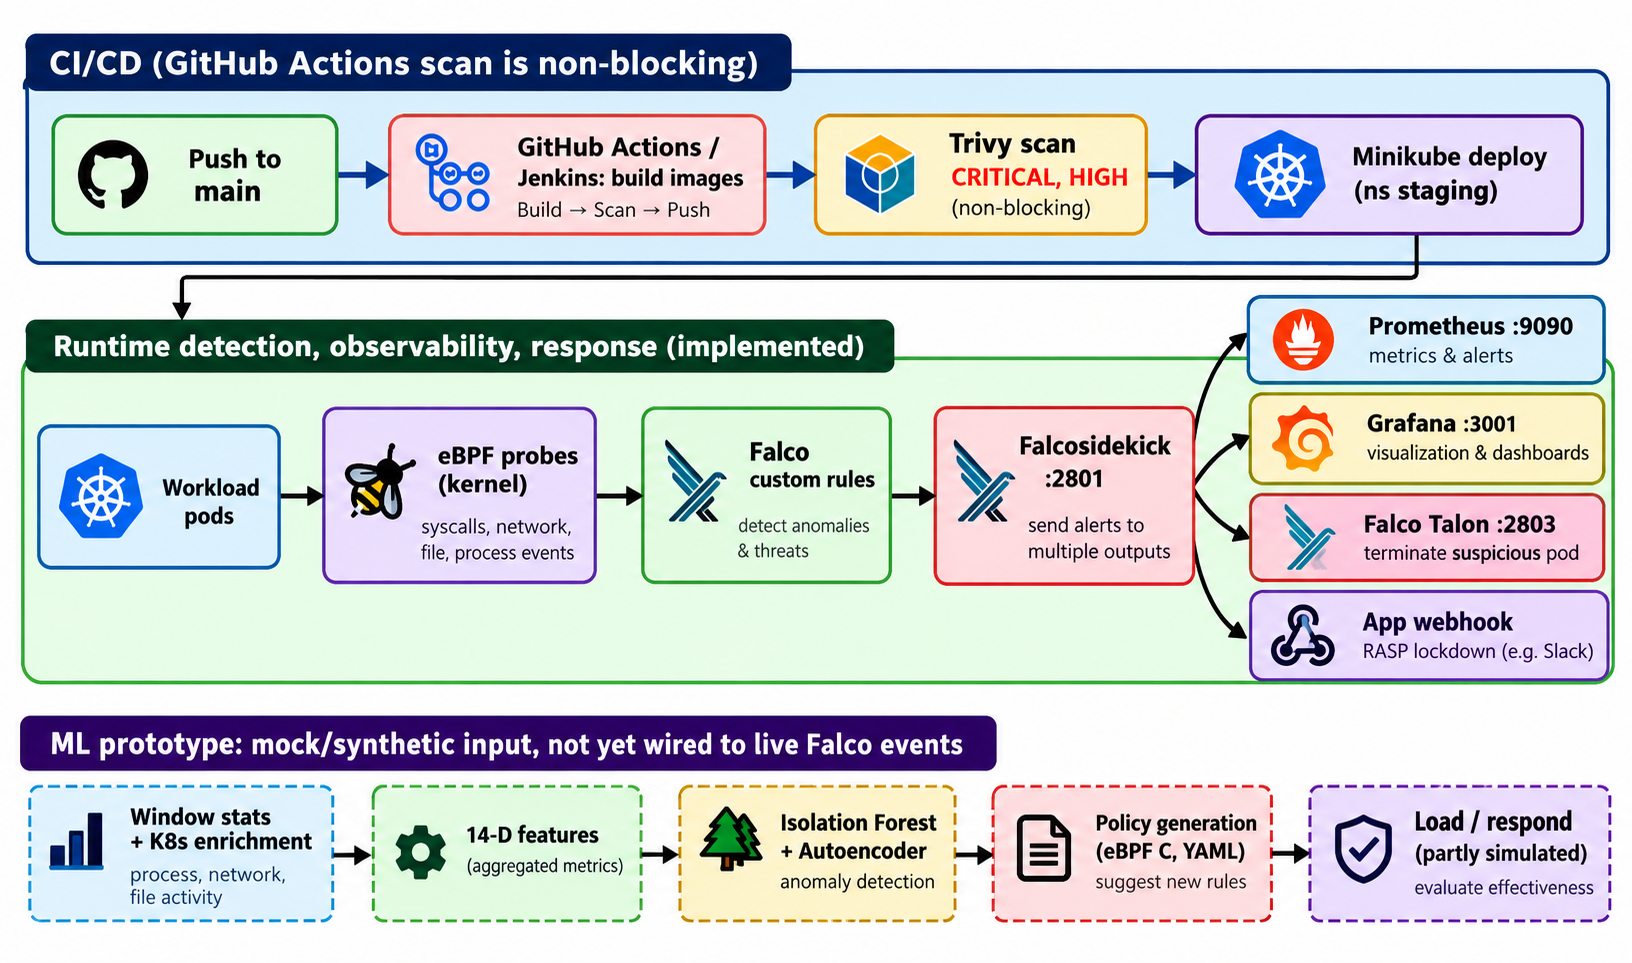
\includegraphics[width=\columnwidth]{fig_arch.png}
\caption{Architecture. Green: implemented. Yellow dashed: prototype code, exercised on mock or synthetic inputs and partly simulated. The two in-kernel enforcers (Tetragon, KubeArmor) plug into the same workload pods as additional response layers.}
\label{fig:arch}
\end{figure}

\subsection{Alert-to-Containment Flow}
For a runtime event the sequence is: (1) the attack request reaches the backend at time $t_\text{action}$; (2)~the process in the container issues a monitored system call; (3)~the eBPF probe delivers the event to Falco, which matches a rule and emits an alert; (4)~Falcosidekick receives the alert at $t_\text{alert}$; (5)~the alert reaches Talon; (6)~Talon calls the Kubernetes API to delete the pod, at $t_\text{terminated}$; (7)~Kubernetes schedules a replacement pod. These timestamps define the latency metrics in Section~\ref{sec:method}. Steps~4--6 involve network hops between processes, which is why we measure each separately rather than assuming equal delivery delay. For the in-kernel mechanisms, the kill happens inside step~2 and is recorded by Tetragon to the nanosecond.

\section{Implementation}\label{sec:impl}
\subsection{CI/CD Stage}
A GitHub Actions workflow runs on pushes and pull requests to \texttt{main}. It builds Docker images for the backend and frontend and runs Trivy against each, reporting CRITICAL and HIGH findings with unfixed vulnerabilities ignored. The exit code is set to zero, so findings are reported but never fail the build; a gate on fixable CRITICAL findings is future work (Section~\ref{sec:road}). A Jenkins pipeline implements a second CI/CD path.

\subsection{Deployment and Workload}
The application is a full-stack web app: a static HTML/CSS/JavaScript frontend served by nginx, and a Node.js/Express backend. The backend runs as a non-root user (UID~10001) with privilege escalation disabled and two replicas behind a Service. The testbed is an HP~280 Pro G6, Ubuntu~22.04 LTS (kernel~6.8), k3s~v1.36 with Helm, on a single dedicated node. The security stack is Falco~0.45 (modern eBPF), Falcosidekick, Falco Talon~0.3, Tetragon~1.7.1, and the KubeArmor operator~v1.7.5 (AppArmor enforcer, as the BPF-LSM is not enabled on this host).

\subsection{Detection Rules and Response Mechanisms}
Two custom Falco rules target the backend container (Table~\ref{tab:rules}); Falco's default rule set also fires during the realistic suite. Six response mechanisms are compared (Table~\ref{tab:mech}). M3 and M4 enforce the same two behaviours the custom rules detect, as policies applied before the pods start, so Falco keeps detecting under every mechanism. Two limits found on the testbed shape M4: on the Alpine image \texttt{/bin/sh} is a symlink to \texttt{/bin/busybox} and AppArmor matches the resolved path, so blocking a shell means blocking every BusyBox tool; and the first program started by \texttt{kubectl exec} runs before the container's AppArmor profile applies, so the attacker's entry shell starts and only the programs it then runs are refused.

\begin{table}[t]
\caption{Custom Falco detection rules}
\label{tab:rules}
\centering
\begin{tabular}{@{}p{0.30\columnwidth}p{0.14\columnwidth}p{0.42\columnwidth}@{}}
\toprule
Rule & Priority & Trigger\\
\midrule
Shell Spawned in Eval Backend & WARNING & A shell process starts in the backend container\\
Sensitive Path Open in Eval Backend & CRITICAL & \texttt{open*} on \texttt{/etc/shadow} or \texttt{/bin/hack}, success or failure\\
\bottomrule
\end{tabular}
\end{table}

\begin{table}[t]
\caption{Response mechanisms compared}
\label{tab:mech}
\centering
\begin{tabular}{@{}cp{0.74\columnwidth}@{}}
\toprule
ID & Response on detection\\
\midrule
M0 & None (detect-only baseline)\\
M1 & Falco Talon deletes the pod (\texttt{kubernetes:terminate}, grace~0); the Deployment recreates it\\
M2 & Talon creates an egress-blocking NetworkPolicy for all replicas\\
M3 & Tetragon sends \texttt{SIGKILL} in the kernel to any backend process that starts a shell or opens \texttt{/etc/shadow} or \texttt{/bin/hack}\\
M4 & KubeArmor (AppArmor) refuses to run \texttt{/bin/busybox} and to open \texttt{/etc/shadow} or \texttt{/bin/hack}\\
M5 & In-app RASP returns 403 on threat routes for 30\,s after 3 threat requests\\
\bottomrule
\end{tabular}
\end{table}

\section{Planned Learned-Scoring Layer (Future Work)}\label{sec:ml}
Beyond the rule-based detection evaluated above, the \texttt{ml\_pipeline/} directory contains a design for a learned-scoring layer. We describe it here as \emph{future work}; it is not among the measured results of this paper. The motivation is that static rules only catch what their authors anticipated; a model of normal behaviour could raise a score for activity no rule describes, at the cost of false positives and a dependence on representative training data. In the planned design, events are parsed from JSON, enriched with pod and namespace, and held in a per-container sliding window of up to 100 events. Window statistics map to a 14-dimensional vector (syscall frequency, unique syscalls, file-access rate, unique files, sensitive-file count, network connections, unique ports, outbound bytes, process executions, unique processes, process-tree depth, CPU, memory, I/O~wait). An isolation forest (100 trees, contamination~0.05) and a PyTorch autoencoder (14--32--16--4--16--32--14, Adam, 100 epochs) score each window. The isolation forest scores a sample $x$ by its expected path length across the trees~\cite{iforest}:
\begin{equation}
s(x,n)=2^{-E[h(x)]/c(n)},\quad c(n)=2H(n-1)-\frac{2(n-1)}{n},
\end{equation}
where $h(x)$ is the path length, $n$ the subsample size, and $H(\cdot)$ the harmonic number. Scores near~1 indicate anomalies. The autoencoder score is the mean squared reconstruction error over the 14 features,
\begin{equation}
e(x)=\frac{1}{14}\sum_{i=1}^{14}\left(x_i-\hat{x}_i\right)^2 ,
\end{equation}
and the two scores are averaged and mapped to LOW/MEDIUM/HIGH/CRITICAL. Evaluating this layer is deferred to future work (Section~\ref{sec:road}): the current code runs only on synthetic data (105 samples), has not been exercised on live Falco events, and no accuracy is claimed for it here.

\section{Implementation Status}\label{sec:status}
Table~\ref{tab:impl} states the boundary between what is built and exercised with measurements, and what is a prototype on synthetic input. The runtime detection, forwarding, observability, and all six response mechanisms are implemented and measured; the learned-scoring layer is future work, exercised only on synthetic data.

\begin{table}[t]
\caption{Implementation status}
\label{tab:impl}
\centering
\begin{tabular}{@{}p{0.40\columnwidth}p{0.46\columnwidth}@{}}
\toprule
Component & Status\\
\midrule
Image build, Trivy scan & Implemented; non-blocking\\
Jenkins / GitHub Actions & Implemented\\
k3s deployment, workload & Implemented\\
Falco eBPF + custom rules & Implemented; measured\\
Falcosidekick fan-out & Implemented; measured\\
Talon M1/M2, Tetragon M3, KubeArmor M4, RASP M5 & Implemented; measured\\
Prometheus, Grafana, Loki & Implemented\\
Learned-scoring layer & Future work, synthetic input\\
\bottomrule
\end{tabular}
\end{table}

\section{Evaluation Methodology}\label{sec:method}
\subsection{Scenarios}
Three attack scenarios and two load-only scenarios are used. \emph{s1-exec}: \texttt{kubectl exec} into the target pod, then eight discovery and sensitive-path steps 1\,s apart. \emph{s2-http}: eight calls to the application's \texttt{/api/threat/*} endpoints (the only scenario M5 reacts to). \emph{s3-abuse}: one public endpoint triggered at 6, 30, or 120 times per minute for 300\,s. \emph{s4-realistic}: 13 Falco event-generator \texttt{syscall} actions run inside the container, each tagged with a MITRE ATT\&CK for Containers technique, covering credential access, execution, defense evasion, discovery, and privilege escalation. \emph{s0-benign} is normal traffic only, for false positives.

Every attack step sends a beacon to a collector running on the host, outside the cluster. Falco alerts (via Falcosidekick) and Talon actions reach the same collector, so all timestamps come from one host clock. A benign load runs through the Service during every run. The realistic suite uses an established public tool rather than hand-written scripts; its binary is built statically (CGO-free) so it runs in the Alpine container, where the attack must execute to trip the container-scoped policies.

\subsection{Latency Formulas}
With $t_\text{action}$ the time the attack request is issued and $t_\text{alert}$ the time the alert reaches Falcosidekick, detection latency is
\begin{equation}
L_\text{det}=t_\text{alert}-t_\text{action}.
\end{equation}
For the Kubernetes-level responses, containment latency is taken from the Talon completion notification,
\begin{equation}
L_\text{cont}=t_\text{terminated}-t_\text{action}.
\end{equation}
The pod being gone from the Kubernetes API does not mean its processes have stopped. For the in-kernel mechanism we therefore also record, from Tetragon's nanosecond process events, the first kill and the exit of the attacker's interactive shell:
\begin{equation}
L_\text{kill}=t_\text{SIGKILL}-t_\text{action},\quad
L_\text{sess}=t_\text{exit}^{\,\text{shell}}-t_\text{action}.
\end{equation}
Detection and false-positive rate are
\begin{equation}
\mathrm{DR}=\frac{TP}{TP+FN}\times100,\qquad
\mathrm{FPR}=\frac{FP}{FP+TN}\times100.
\end{equation}

\subsection{Statistics}
Each applicable (mechanism, scenario) pair is run 20~times (abuse: 5 per rate; overhead: 10 windows per level) on fresh pods, with no runs discarded. We report the median and a 95\,\% confidence interval. The median and percentiles use the nearest-rank definition: for $n$ sorted samples $x_{(1)}\le\dots\le x_{(n)}$, the $p$-th percentile is
\begin{equation}
P_p = x_{(k)},\qquad k=\mathrm{ceil}\!\left(\frac{p\,n}{100}\right),
\end{equation}
where $\mathrm{ceil}(\cdot)$ rounds up to the next integer.
The confidence interval is a percentile bootstrap: drawing $B=2000$ resamples $\{x^{*b}\}$ of size $n$ with replacement and taking the median of each, the interval is
\begin{equation}
\left[\,Q_{2.5\%}\!\left(\{\tilde{x}^{*b}\}\right),\; Q_{97.5\%}\!\left(\{\tilde{x}^{*b}\}\right)\right],\quad \tilde{x}^{*b}=\mathrm{median}(x^{*b}).
\end{equation}

\subsection{Abuse and Overhead Metrics}
For the abuse scenario we bin the benign traffic into 1\,s windows. Writing $r_b=\text{ok}(b)/\text{total}(b)$ for the success fraction in bin $b$, the unavailability $U$ (in seconds) is the number of 1\,s bins with
\begin{equation}
r_b < 0.5 .
\end{equation}
For the overhead experiment, benign load only, we read each agent pod's CPU time from the cgroup \texttt{cpu.stat} (\texttt{usage\_usec}) and memory from \texttt{memory.current}, and host CPU from \texttt{/proc/stat}. Over a window of length $\Delta t$ the agents' CPU in cores and the host utilization are
\begin{equation}
C_\text{agents}=\sum_{p\in\text{agents}}\frac{\Delta u_p}{10^{6}\,\Delta t},\qquad
U_\text{host}=1-\frac{\Delta\,\text{idle}}{\Delta\,\text{total}} .
\end{equation}
The kernel bills eBPF work to the process that triggers the syscall, so Tetragon's own pod shows almost no CPU and its cost appears in the application's CPU and latency instead.

\section{Results}\label{sec:results}
All experiments ran on the testbed of Section~\ref{sec:impl}; 460 attack and abuse runs plus 200 overhead windows, none failed. Table~\ref{tab:score} summarises the outcome: each mechanism is graded across the five dimensions the rest of this section measures. No mechanism is strong on all five, which is the paper's central result and the argument for a layered response; the subsections and Tables~\ref{tab:cont}--\ref{tab:rq6} give the numbers behind each grade.

\begin{table*}[t]
\caption{Per-mechanism scorecard across the five measured dimensions. Grades are relative to the other mechanisms and summarise the numeric results below: Good, Fair, Poor. M0 is the detect-only baseline and takes no containment action. No mechanism is Good on all five, which is the paper's central argument for a layered response.}
\label{tab:score}
\centering
\setlength{\tabcolsep}{4.5pt}
\begin{tabular}{clcccccl}
\toprule
ID & Mechanism & Speed & Durability & Evidence & Abuse-resistance & Cost & One-line takeaway\\
\midrule
M0  & Detect-only (Falco)   & --   & --   & Good & --   & Good & Sees everything, stops nothing (baseline)\\
M1  & Talon pod terminate   & Fair & Poor & Poor & Fair & Good & Fast API call, but process lives $\sim$2\,s and re-compromises\\
M1g & Talon + replica guard & Fair & Poor & Poor & Good & Good & As M1, but the replica guard removes the self-DoS\\
M2  & Talon egress policy   & Good & Fair & Good & Good & Good & Cuts outbound only; no effect on inbound attacks\\
M3  & Tetragon kernel kill  & Good & Good & Poor & Poor & Good & Fastest and surgical, but abusable and leaves no evidence\\
M4  & KubeArmor LSM block   & Fair & Good & Good & Good & Poor & Keeps workload and logs, but the most expensive\\
M5  & In-app RASP           & Good & Fair & Fair & Good & Good & Guards app-routed attacks; blind to OS-level ones\\
\bottomrule
\end{tabular}
\end{table*}

\subsection{Detection and Containment (s1, s2)}
Falco alerted about 2\,ms after the kernel event whenever the attack executed (the kernel-to-alert pipeline; the raw $L_\text{det}$ for \texttt{s1} additionally includes the $\approx$0.09\,s that \texttt{kubectl exec} takes to start). Table~\ref{tab:cont} gives the containment results. Pod termination (M1) \emph{looks} instant in the Kubernetes API but is not: Talon acts in 0.02--0.10\,s, yet the attacker's shell keeps running until 2.11\,s in the exec attack and the server process until 2.03\,s in the HTTP attack, in every run; the replacement pod is ready in about 1.1\,s and is re-compromised every time, and the attacked pod's logs are lost every time. In-kernel termination (M3) kills the attacker's shell 0.09\,s after the attack starts, with no step completed, no re-compromise, and the evidence kept; in the HTTP attack it kills the server process itself, costing normal users 0.8\,\% errors while the pod restarts. LSM blocking (M4) lets the entry shell start but refuses every command it runs; the first refusal lands at 0.50\,s (exec) and the first block alert at 1.01\,s (HTTP). Network isolation (M2) stops the exec attacker after one step but does nothing against the inbound HTTP attack (Fig.~\ref{fig:steps}), because Talon blocks only outbound traffic.

\begin{table*}[t]
\caption{Containment results, median of 20 runs; 95\,\% bootstrap CIs in parentheses. $L_\text{cont}$ is measured from the Kubernetes API event (M1/M2), the first kernel kill (M3), or the first refusal/block alert (M4); ``active until'' is the attacker's last recorded live moment (session-end beacon). Latency and session-end were instrumented in the phase-2 batches (M0/M1/M3/M4) and the phase-1 batch (M2/M5); the s2 (HTTP) phase-2 batch did not record a session-end for M0, shown ``--''. For s1/M4, 8 steps were \emph{reached} (shell alive) but every command was refused (0 completed).}
\label{tab:cont}
\centering
\begin{tabular}{llllrc}
\toprule
Scn & Mech & $L_\text{cont}$ (s) & Active until (s) & Steps /8 & Re-comp.\\
\midrule
s1 & M0 & --                   & 11.22 (11.00--11.32) & 8 & --\\
s1 & M1 & 0.101 (0.100--0.103) & 2.112 (2.109--2.116) & 2 & 100\,\%\\
s1 & M2 & 0.101 (0.098--0.104) & --                   & 1 & --\\
s1 & M3 & 0.090 (0.088--0.092) & 0.090 (0.088--0.092) & 0 & 0\,\%\\
s1 & M4 & 0.497 (0.480--0.506) & 2.83 (2.82--2.87)    & 0 & 0\,\%\\
\midrule
s2 & M0 & --                   & --                   & 8 & --\\
s2 & M1 & 0.020 (0.017--0.022) & 2.028 (2.027--2.030) & 3 & 100\,\%\\
s2 & M2 & 0.022 (0.017--0.022) & --                   & 8 & --\\
s2 & M3 & 0.008 (0.008--0.008) & 1.015 (1.015--1.016) & 0 & 0\,\%\\
s2 & M4 & 1.008 (1.008--1.009) & --                   & 5 & 0\,\%\\
s2 & M5 & --                   & --                   & 3 & yes\\
\bottomrule
\end{tabular}
\end{table*}

\begin{figure}[t]
\centering
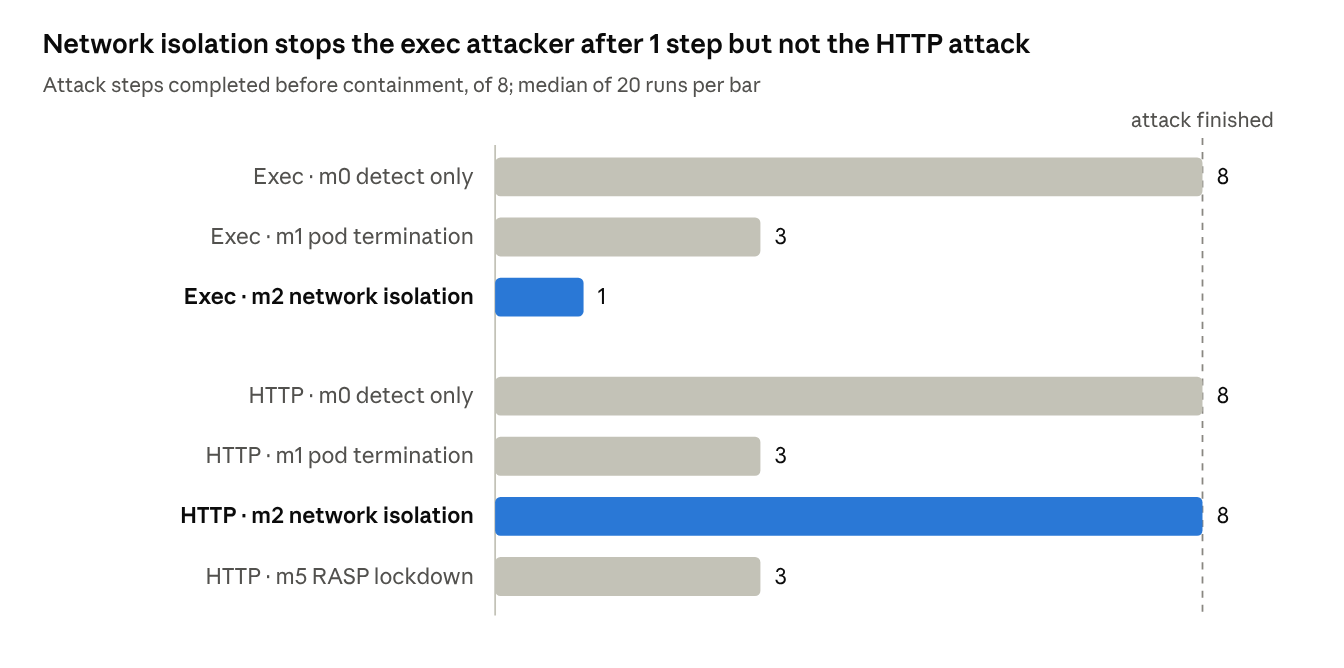
\includegraphics[width=\columnwidth]{fig_steps.png}
\caption{Attack steps completed before containment (of 8), median of 20 runs. Network isolation (M2) stops the exec attacker after one step but not the inbound HTTP attack.}
\label{fig:steps}
\end{figure}

\subsection{Abuse of the Response (RQ4)}
Because M1 and M3 take normal traffic down by design when triggered repeatedly, we measured an outside attacker calling a public endpoint that trips the rule, at 6, 30, or 120 times per minute for 300\,s (Fig.~\ref{fig:abuse}). In-kernel termination is the easiest to abuse: at only 6 triggers per minute it kept the service unavailable 225 of 300\,s, because each trigger kills the server and Kubernetes' restart back-off grows; at 120 per minute the service was down the whole period. Pod termination stayed fully available up to 30 triggers per minute and lost 14\,s at 120 per minute, and adding a minimum-healthy-replicas guard (M1g) removed that outage entirely (0\,s down at every rate). This finding applies whenever an attacker can trigger the monitored behaviour remotely, for example through a remote code-execution foothold they already hold or a legitimate request path that matches a response rule; an application that exposes no such path is not exposed to this particular abuse.

\begin{figure}[t]
\centering
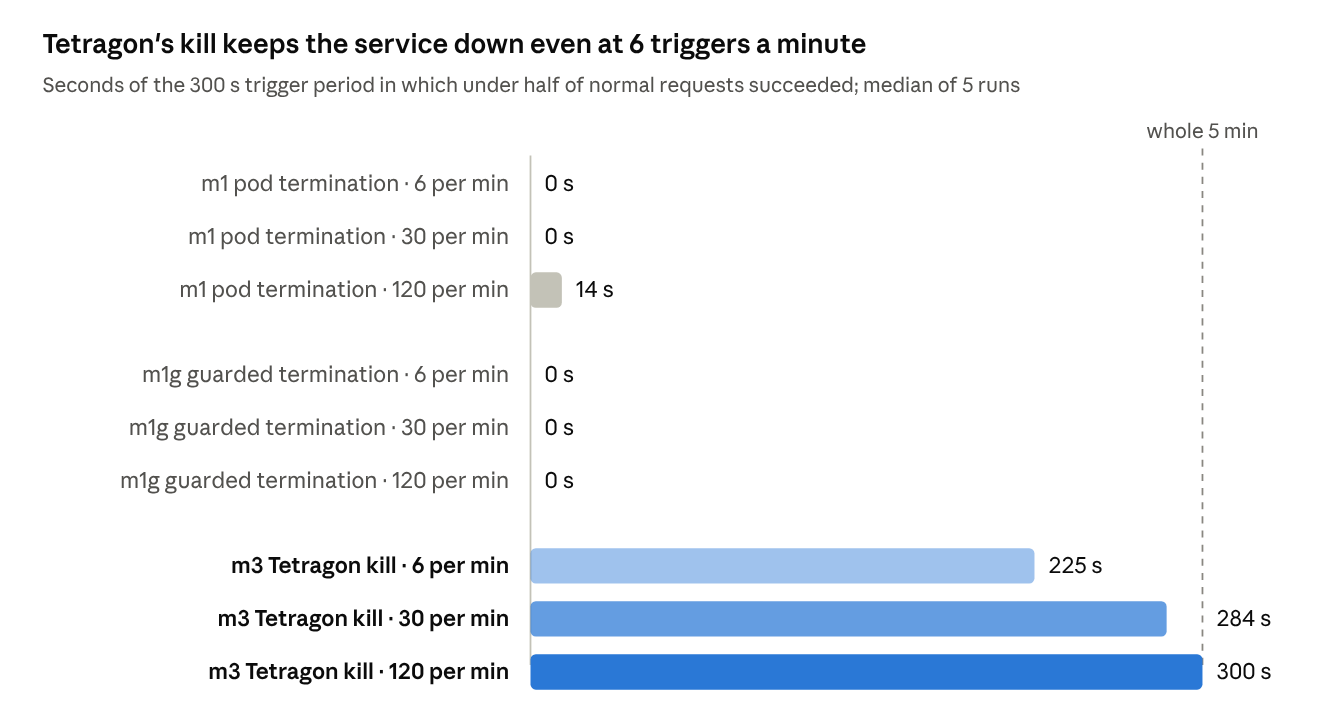
\includegraphics[width=\columnwidth]{fig_abuse.png}
\caption{Seconds of the 300\,s trigger period in which fewer than half of the benign requests succeeded, median of 5 runs. The fastest response is the easiest to abuse.}
\label{fig:abuse}
\end{figure}

\subsection{Steady-State Overhead (RQ5)}
Under benign load only, we compared five stacks (no tools; Falco+Talon; Tetragon; KubeArmor; Falco+Tetragon) at 0/500/1{,}500/2{,}500 requests/s, 10 windows of 60\,s each (Table~\ref{tab:over}, Fig.~\ref{fig:over}). Tetragon's cost was within measurement noise; Falco+Talon added about 0.16 cores of whole-host CPU (0.044 cores in the agent pod itself, Table~\ref{tab:over}) and 0.27\,ms of p99 latency; KubeArmor with default visibility used about 1.2 extra cores of whole-host CPU (0.766 cores in the agent pod) and nearly tripled p99 latency. Whole-host figures come from Fig.~\ref{fig:over}; per-pod figures from Table~\ref{tab:over}. No stack caused request errors. The 500\,requests/s level is confounded by CPU frequency scaling and is excluded from the comparison.

\begin{table}[t]
\caption{Overhead at 2{,}500 requests/s vs.\ no tools (host p99 0.77\,ms), median of 10 windows.}
\label{tab:over}
\centering
\begin{tabular}{@{}lrrr@{}}
\toprule
Stack & Agents CPU (cores) & Agents mem (MB) & p99 (ms)\\
\midrule
Falco + Talon       & 0.044 & 203 & 1.04\\
Tetragon            & 0.001 & 85  & 0.82\\
KubeArmor           & 0.766 & 154 & 2.21\\
Falco + Tetragon    & 0.045 & 293 & 1.18\\
\bottomrule
\end{tabular}
\end{table}

\begin{figure}[t]
\centering
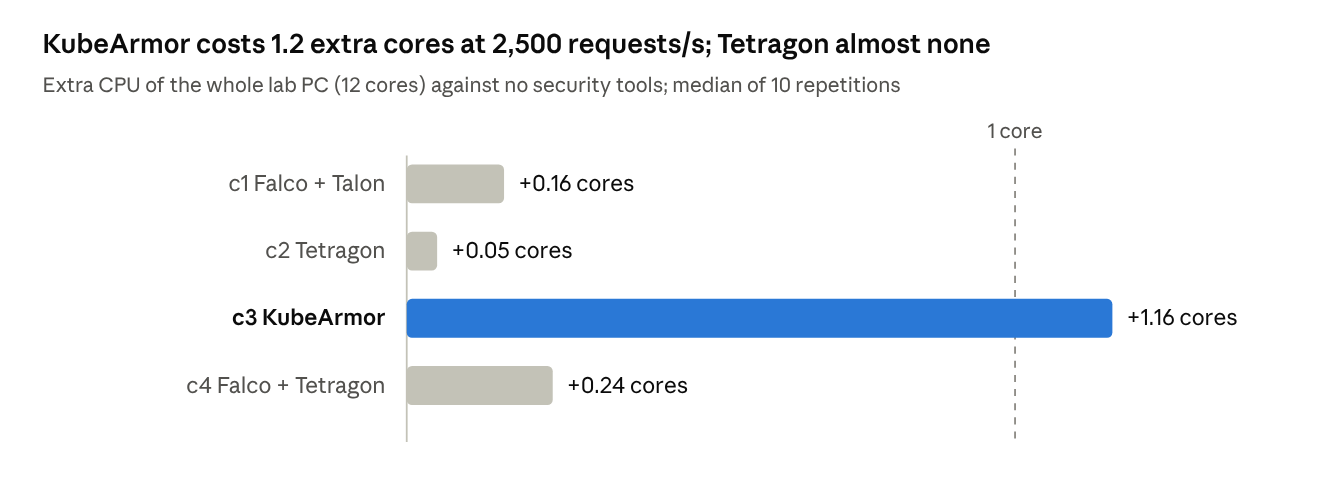
\includegraphics[width=\columnwidth]{fig_overhead.png}
\caption{Extra whole-host CPU against no security tools at 2{,}500 requests/s, median of 10 repetitions. The overhead ranking inverts the protection ranking.}
\label{fig:over}
\end{figure}

\subsection{Realistic Attacks (RQ6)}
To answer the concern that the attacks were self-written, we ran an established public suite: 13 Falco event-generator \texttt{syscall} actions, each mapped to a MITRE ATT\&CK technique, inside the target container as its non-root user; 100 runs, none failed (Table~\ref{tab:rq6}). Falco fired real default rules across the suite (fileless/\texttt{memfd} execution, \texttt{ptrace}, symlink and hardlink over sensitive files, credential and private-key searches, \texttt{/dev/shm} execution) plus the two custom rules. The suite reproduced the mechanism ranking: Tetragon (M3) killed the attacker's shell on spawn at 0.50\,s, so none of the 13 actions ran; KubeArmor (M4) let the actions run but refused each sensitive open or exec; Talon (M1) let about one action through before deleting the pod; and in-app RASP (M5) was blind to the syscall-level attacks and behaved like the detect-only baseline. Two observations follow: under M3 the shell dies so early that Falco has nothing left to report (detection and in-kernel kill trade off), and the per-action detection figure for M1 is inflated by time-window attribution, so the reliable figures are the session-level ones.

\begin{table}[t]
\caption{Realistic suite (RQ6), 13 MITRE-tagged actions, 100 runs.}
\label{tab:rq6}
\centering
\begin{tabular}{@{}lccl@{}}
\toprule
Mech & Actions ran & Falco detected & Containment\\
\midrule
M0 detect only   & 13/13 & 100\,\% & none\\
M1 Talon term.   & $\approx$1/13 & yes & pod deleted $\approx$0.52\,s\\
M3 Tetragon kill & 0/13  & n/a & shell killed on spawn 0.50\,s\\
M4 KubeArmor     & 13/13 & 100\,\% & each op refused; block 0.93\,s\\
M5 in-app RASP   & 13/13 & 100\,\% & none (blind to syscalls)\\
\bottomrule
\end{tabular}
\end{table}

\section{Discussion}\label{sec:discuss}
\subsection{What the Measurements Show}
No single response wins on every measure (Table~\ref{tab:score}), which supports a layered design. The central, non-obvious result is the gap between \emph{API-level} and \emph{process-level} containment: deleting a pod returns from the Kubernetes API in tens of milliseconds, but the attacker's process keeps running for about two seconds, long enough to finish a multi-step action and to be re-compromised on the replacement pod. In-kernel termination removes that gap but is the most abusable and, by stopping the attack at the first syscall, leaves the detection pipeline nothing to log. KubeArmor contains without killing (the shell stays alive but achieves nothing), which keeps the workload and its evidence but costs the most to run.

\subsection{Rules versus Learned Scoring}
Rule-based detection is precise and explainable, but only detects what someone wrote a rule for. A learned layer could flag unusual combinations of activity, at the cost of explainability and a dependence on representative benign data. Our position is that the learned layer should first run in an advisory role, raising tickets, and should not trigger automated enforcement until its false-positive rate on real workloads has been measured.

\subsection{Safety of Automated Response}
Table~\ref{tab:risks} lists response risks and mitigations. The central concern is that a response mechanism is itself an attack surface: an attacker who can make benign pods trip a termination rule turns the defence into a denial-of-service tool. Rate limits per deployment, a minimum number of healthy replicas before termination (measured here as M1g), and escalation from log-only all reduce this.

\begin{table}[t]
\caption{Automated-response risks and mitigations}
\label{tab:risks}
\centering
\begin{tabular}{@{}p{0.40\columnwidth}p{0.46\columnwidth}@{}}
\toprule
Risk & Mitigation\\
\midrule
False positive terminates a healthy pod & Dry-run first; require replicas $>1$; per-deployment rate limit\\
Attacker induces terminations (DoS) & De-duplication; cool-down; minimum healthy replicas (M1g)\\
Evidence lost with the pod & Ship logs to Loki before termination\\
Untrusted identifiers in generated policy & Fixed templates; strict validation\\
Host process signalling & Use API-level or in-kernel actions, not raw PID signals\\
\bottomrule
\end{tabular}
\end{table}

\section{Limitations}\label{sec:limits}
\begin{itemize}
\item \textbf{Single node, one application.} Evaluation is single-node k3s with one full-stack app; multi-node behaviour is untested.
\item \textbf{Policies match the attack behaviours.} The M3/M4 policies target the shell-spawn and sensitive-file behaviours the suite also exercises, so this measures mechanism behaviour, not policy-authoring difficulty.
\item \textbf{Overhead is one light workload.} The app does little work per request; the 500\,requests/s level is confounded by CPU power saving, and KubeArmor was measured only at default visibility.
\item \textbf{LSM back end.} KubeArmor used AppArmor, not BPF-LSM, on this host; the symlink and \texttt{kubectl exec} entry-process effects are AppArmor-specific.
\item \textbf{Attack entry via \texttt{kubectl exec}.} The \texttt{s1} scenario enters the container with \texttt{kubectl exec}, which presumes cluster credentials and so sits outside the in-container code-execution threat model; we use it only as a stand-in for an interactive shell obtained by other means, and note that the AppArmor entry-process effect in M4 is specific to this entry path.
\item \textbf{Learned-scoring layer is future work.} It is presented as a design only; the code has run on synthetic data alone, not on real captured telemetry, and no accuracy is claimed.
\item \textbf{Zero false positives} is expected from two narrowly scoped rules and says little about real workloads.
\end{itemize}

\section{Roadmap}\label{sec:road}
The next steps, in order: make the Trivy stage a gate on fixable CRITICAL findings; feed the ML layer from captured Falco events with feature standardisation fixed at training time, then measure precision/recall on a labelled benign/attack set under this protocol; constrain generated eBPF programs to a validated template, compile and verify before enforcement; and package the agent as a DaemonSet to repeat the evaluation on a multi-node cluster.

\section{Data and Code Availability}
All mechanism configurations and policies, the measurement harness and attack scenarios, and the raw per-run data behind every table and figure are released at \url{https://github.com/Naveen4421/real_time_security_using_ebpf}. A tagged release accompanies this paper so that the exact artifacts used here can be retrieved.

\section{Conclusion}
The repository demonstrates a working path from commit to containment, and this paper measures the containment step directly. Across five containment mechanisms and a detect-only baseline, detection is fast and cheap, but containment behaviour diverges sharply: pod termination hides a multi-second process-level gap and loses evidence; in-kernel termination is immediate but the most abusable and blinds detection; LSM blocking contains without killing but costs the most; and in-application protection misses OS-level attacks. No mechanism wins on speed, durability, evidence, abuse-resistance, and cost together, so a layered response, chosen per workload, is the practical recommendation. All configurations, scripts, and raw run data are released for reproduction.

\balance
\begin{thebibliography}{99}
\bibitem{iforest} F.~T. Liu, K.~M. Ting, and Z.-H. Zhou, ``Isolation forest,'' in \emph{Proc. IEEE Int. Conf. Data Mining (ICDM)}, 2008, pp.~413--422, doi:\,10.1109/ICDM.2008.17.
\bibitem{chernyshev2021} M.~Chernyshev, Z.~Baig, and S.~Zeadally, ``Cloud-native application security: Risks, opportunities, and challenges in securing the evolving attack surface,'' \emph{Computer}, vol.~54, no.~11, pp.~47--57, 2021, doi:\,10.1109/MC.2021.3076537.
\bibitem{zhang2023} Z.~Zhang and L.~Chen, ``Anomaly detection model for process resource usage in hybrid system based on eBPF and isolation forest,'' in \emph{Proc. 6th Int. Conf. Artif. Intell. Pattern Recognit. (AIPR)}, 2023, doi:\,10.1145/3641584.3641812.
\bibitem{her2025} J.~Her, J.~Kim, J.~Kim, and S.~Lee, ``An in-depth analysis of eBPF-based system security tools in cloud-native environments,'' \emph{IEEE Access}, vol.~13, pp.~155588--155604, 2025, doi:\,10.1109/ACCESS.2025.3605432.
\bibitem{anand2025} N.~Anand, M.~A. Saifulla, P.~K. Aakula, R.~B. Ponnuru, R.~Patan, and C.~R.~P. Reddy, ``Enhancing intrusion detection against denial of service and distributed denial of service attacks leveraging extended Berkeley packet filter and machine learning algorithms,'' \emph{IET Commun.}, vol.~19, no.~1, art.~e12879, 2025.
\bibitem{ghimire2025} S.~Ghimire, N.~Bhurtel, R.~Sahani, and S.~Jha, ``eBPF-PATROL: Protective agent for threat recognition and overreach limitation using eBPF in containerized and virtualized environments,'' arXiv:2511.18155, 2025.
\bibitem{rezvani2024} M.~Rezvani, A.~Jahanshahi, and D.~Wong, ``Characterizing in-kernel observability of latency-sensitive request-level metrics with eBPF,'' in \emph{Proc. IEEE Int. Symp. Performance Analysis of Systems and Software (ISPASS)}, 2024, pp.~24--35.
\bibitem{syairozi2025} A.~A. Syairozi and Arizal, ``Comparative analysis of eBPF-based runtime security monitoring tools in monitoring and threat detection on Kubernetes,'' in \emph{Proc. 1st RITECH}, 2025, pp.~136--141, doi:\,10.5220/0014272700004928.
\bibitem{lin2018} X.~Lin, L.~Lei, Y.~Wang, J.~Jing, K.~Sun, and Q.~Zhou, ``A measurement study on Linux container security: Attacks and countermeasures,'' in \emph{Proc. 34th Annu. Computer Security Applications Conf. (ACSAC)}, 2018, pp.~418--429, doi:\,10.1145/3274694.3274720.
\bibitem{wong2023} A.~Y. Wong, E.~G. Chekole, M.~Ochoa, and J.~Zhou, ``On the security of containers: Threat modeling, attack analysis, and mitigation strategies,'' \emph{Comput. Secur.}, vol.~128, art.~103140, 2023, doi:\,10.1016/j.cose.2023.103140.
\bibitem{haq2024} M.~S. Haq, T.~D. Nguyen, A.~S. Tosun, F.~Vollmer, T.~Korkmaz, and A.-R. Sadeghi, ``SoK: A comprehensive analysis and evaluation of Docker container attack and defense mechanisms,'' in \emph{Proc. IEEE Symp. Security and Privacy (S\&P)}, 2024.
\bibitem{abbas2022} M.~Abbas, S.~Khan, A.~Monum, F.~Zaffar, R.~Tahir, D.~Eyers, H.~Irshad, A.~Gehani, V.~Yegneswaran, and T.~Pasquier, ``PACED: Provenance-based automated container escape detection,'' in \emph{Proc. IEEE Int. Conf. Cloud Engineering (IC2E)}, 2022, pp.~261--272, doi:\,10.1109/IC2E55432.2022.00035.
\bibitem{elkhairi2022} A.~El Khairi, M.~Caselli, C.~Knierim, A.~Peter, and A.~Continella, ``Contextualizing system calls in containers for anomaly-based intrusion detection,'' in \emph{Proc. ACM Cloud Computing Security Workshop (CCSW)}, 2022, doi:\,10.1145/3560810.3564266.
\bibitem{liu2018} M.~Liu, Z.~Xue, X.~Xu, C.~Zhong, and J.~Chen, ``Host-based intrusion detection system with system calls: Review and future trends,'' \emph{ACM Comput. Surv.}, vol.~51, no.~5, art.~98, 2018, doi:\,10.1145/3214304.
\bibitem{bridges2019} R.~A. Bridges, T.~R. Glass-Vanderlan, M.~D. Iannacone, M.~S. Vincent, and Q.~Chen, ``A survey of intrusion detection systems leveraging host data,'' \emph{ACM Comput. Surv.}, vol.~52, no.~6, art.~128, 2019.
\bibitem{chen2024} K.~Chen, Y.~Zhao, J.~Guo, Z.~Gu, L.~Han, and K.~Tang, ``A container escape detection method based on a dependency graph,'' \emph{Electronics}, vol.~13, no.~23, art.~4773, 2024, doi:\,10.3390/electronics13234773.
\bibitem{cisar2016} P.~\v{C}isar and S.~Maravi\'{c}-\v{C}isar, ``The framework of runtime application self-protection technology,'' in \emph{Proc. IEEE 17th Int. Symp. Computational Intelligence and Informatics (CINTI)}, 2016, pp.~81--85, doi:\,10.1109/CINTI.2016.7846383.
\bibitem{seth2025} A.~Seth, S.~Bhattacharya, S.~Elder, N.~Zahan, and L.~Williams, ``Comparing effectiveness and efficiency of interactive application security testing (IAST) and runtime application self-protection (RASP) tools in a large Java-based system,'' \emph{Empirical Softw. Eng.}, 2025, doi:\,10.1007/s10664-025-10621-5.
\bibitem{ebpf} eBPF Foundation, ``eBPF documentation.'' [Online]. Available: https://ebpf.io (accessed Oct.~2026).
\bibitem{falco} CNCF, ``Falco: Cloud native runtime security,'' version~0.45 (modern-eBPF driver), 2025. [Online]. Available: https://falco.org (accessed Oct.~2026).
\bibitem{falcosidekick} Falco Security, ``Falcosidekick.'' [Online]. Available: https://github.com/falcosecurity/falcosidekick (accessed Oct.~2026).
\bibitem{talon} Falco Security, ``Falco Talon,'' version~0.3, 2025. [Online]. Available: https://github.com/falcosecurity/falco-talon (accessed Oct.~2026).
\bibitem{tetragon} Cilium, ``Tetragon: eBPF-based security observability and runtime enforcement,'' version~1.7.1, 2025. [Online]. Available: https://tetragon.io (accessed Oct.~2026).
\bibitem{kubearmor} KubeArmor Authors, ``KubeArmor: Runtime security enforcement,'' operator version~1.7.5 (AppArmor enforcer), 2025. [Online]. Available: https://kubearmor.io (accessed Oct.~2026).
\bibitem{trivy} Aqua Security, ``Trivy: vulnerability and misconfiguration scanner.'' [Online]. Available: https://github.com/aquasecurity/trivy (accessed Oct.~2026).
\bibitem{prometheus} Prometheus Authors, ``Prometheus monitoring system.'' [Online]. Available: https://prometheus.io (accessed Oct.~2026).
\bibitem{loki} Grafana Labs, ``Grafana Loki.'' [Online]. Available: https://grafana.com/oss/loki (accessed Oct.~2026).
\bibitem{ghactions} GitHub, ``GitHub Actions documentation.'' [Online]. Available: https://docs.github.com/actions (accessed Oct.~2026).
\bibitem{jenkins} Jenkins Project, ``Jenkins.'' [Online]. Available: https://www.jenkins.io (accessed Oct.~2026).
\end{thebibliography}

\end{document}
